\documentclass{standalone}
\usepackage{tikz}
\usepackage{flowchart}
\usetikzlibrary{arrows}
\begin{document}

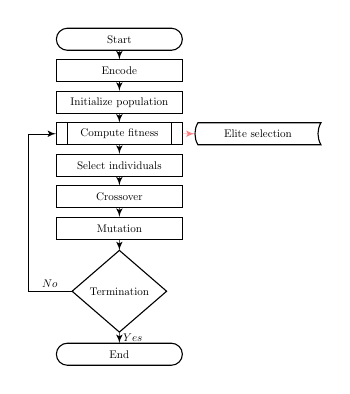
\begin{tikzpicture}[scale=.4, transform shape]
      \begin{scope}[
        every node/.style={draw, minimum width=4cm, minimum height=0.7cm}, 
        node distance=1cm,
        % process/.append style={very thick, draw=blue!50!black!50, top color=white, bottom color=blue!50!black!20},
        % terminal/.append style={very thick,draw=black!50,
        % top color=white,bottom color=black!20,font=\ttfamily},
        %predproc/.append style={very thick,draw=red!50!black!50,top color=white,
        %bottom color=red!50!black!20,font=\itshape},
        ]
        \node (start)      [terminal]{Start};
        \node (encode)     [process,below of =start]{Encode};
        \node (initialize) [process, below of=encode]      {Initialize population};
        \node (fitness)    [predproc, below of=initialize] {Compute fitness};
        \node (reserve)    [storage, right of=fitness, xshift=3.4cm] {Elite selection};
        \node (selection)     [process, below of=fitness]    {Select individuals};
        \node (crossover)  [process, below of=selection]     {Crossover};
        \node (mutate)     [process, below of=crossover]  {Mutation};
        \node (stop)       [decision, minimum width=3cm, below of=mutate, yshift=-1cm]    {Termination};
        \node (end)        [terminal, below of=stop,yshift=-1cm] {End};
      \end{scope}
      \begin{scope}[
        >=latex',
        ]
        \draw[->,ultra thin] (start.south)  -- (encode);
        \draw[->,ultra thin] (encode)       -- (initialize);
        \draw[->,ultra thin] (initialize)   -- (fitness);
        \draw[->,ultra thin] (fitness)      -- (selection);
        \draw[->,ultra thin, red!50,dashed] (fitness.east) -- (reserve.west);
        \draw[->,ultra thin] (selection)       -- (crossover);
        \draw[->,ultra thin] (crossover)    -- (mutate);
        \draw[->,ultra thin] (mutate)       -- (stop);
        
        \draw[->,ultra thin] (stop.west)    -- node[above]{$No$} ++(-1.4cm,0pt) |- (fitness.west);
        \draw[->,ultra thin](stop.south) --node[right]{$Yes$}(end);
      \end{scope}
\end{tikzpicture}
\end{document}
